\documentclass[twoside]{book}

% Packages required by doxygen
\usepackage{fixltx2e}
\usepackage{calc}
\usepackage{doxygen}
\usepackage[export]{adjustbox} % also loads graphicx
\usepackage{graphicx}
\usepackage[utf8]{inputenc}
\usepackage{makeidx}
\usepackage{multicol}
\usepackage{multirow}
\PassOptionsToPackage{warn}{textcomp}
\usepackage{textcomp}
\usepackage[nointegrals]{wasysym}
\usepackage[table]{xcolor}

% Font selection
\usepackage[T1]{fontenc}
\usepackage[scaled=.90]{helvet}
\usepackage{courier}
\usepackage{amssymb}
\usepackage{sectsty}
\renewcommand{\familydefault}{\sfdefault}
\allsectionsfont{%
  \fontseries{bc}\selectfont%
  \color{darkgray}%
}
\renewcommand{\DoxyLabelFont}{%
  \fontseries{bc}\selectfont%
  \color{darkgray}%
}
\newcommand{\+}{\discretionary{\mbox{\scriptsize$\hookleftarrow$}}{}{}}

% Page & text layout
\usepackage{geometry}
\geometry{%
  a4paper,%
  top=2.5cm,%
  bottom=2.5cm,%
  left=2.5cm,%
  right=2.5cm%
}
\tolerance=750
\hfuzz=15pt
\hbadness=750
\setlength{\emergencystretch}{15pt}
\setlength{\parindent}{0cm}
\setlength{\parskip}{3ex plus 2ex minus 2ex}
\makeatletter
\renewcommand{\paragraph}{%
  \@startsection{paragraph}{4}{0ex}{-1.0ex}{1.0ex}{%
    \normalfont\normalsize\bfseries\SS@parafont%
  }%
}
\renewcommand{\subparagraph}{%
  \@startsection{subparagraph}{5}{0ex}{-1.0ex}{1.0ex}{%
    \normalfont\normalsize\bfseries\SS@subparafont%
  }%
}
\makeatother

% Headers & footers
\usepackage{fancyhdr}
\pagestyle{fancyplain}
\fancyhead[LE]{\fancyplain{}{\bfseries\thepage}}
\fancyhead[CE]{\fancyplain{}{}}
\fancyhead[RE]{\fancyplain{}{\bfseries\leftmark}}
\fancyhead[LO]{\fancyplain{}{\bfseries\rightmark}}
\fancyhead[CO]{\fancyplain{}{}}
\fancyhead[RO]{\fancyplain{}{\bfseries\thepage}}
\fancyfoot[LE]{\fancyplain{}{}}
\fancyfoot[CE]{\fancyplain{}{}}
\fancyfoot[RE]{\fancyplain{}{\bfseries\scriptsize Generated by Doxygen }}
\fancyfoot[LO]{\fancyplain{}{\bfseries\scriptsize Generated by Doxygen }}
\fancyfoot[CO]{\fancyplain{}{}}
\fancyfoot[RO]{\fancyplain{}{}}
\renewcommand{\footrulewidth}{0.4pt}
\renewcommand{\chaptermark}[1]{%
  \markboth{#1}{}%
}
\renewcommand{\sectionmark}[1]{%
  \markright{\thesection\ #1}%
}

% Indices & bibliography
\usepackage{natbib}
\usepackage[titles]{tocloft}
\setcounter{tocdepth}{3}
\setcounter{secnumdepth}{5}
\makeindex

% Hyperlinks (required, but should be loaded last)
\usepackage{ifpdf}
\ifpdf
  \usepackage[pdftex,pagebackref=true]{hyperref}
\else
  \usepackage[ps2pdf,pagebackref=true]{hyperref}
\fi
\hypersetup{%
  colorlinks=true,%
  linkcolor=blue,%
  citecolor=blue,%
  unicode%
}

% Custom commands
\newcommand{\clearemptydoublepage}{%
  \newpage{\pagestyle{empty}\cleardoublepage}%
}

\usepackage{caption}
\captionsetup{labelsep=space,justification=centering,font={bf},singlelinecheck=off,skip=4pt,position=top}

%===== C O N T E N T S =====

\begin{document}

% Titlepage & ToC
\hypersetup{pageanchor=false,
             bookmarksnumbered=true,
             pdfencoding=unicode
            }
\pagenumbering{alph}
\begin{titlepage}
\vspace*{7cm}
\begin{center}%
{\Large Bullet\+\_\+hell }\\
\vspace*{1cm}
{\large Generated by Doxygen 1.8.13}\\
\end{center}
\end{titlepage}
\clearemptydoublepage
\pagenumbering{roman}
\tableofcontents
\clearemptydoublepage
\pagenumbering{arabic}
\hypersetup{pageanchor=true}

%--- Begin generated contents ---
\chapter{Hierarchical Index}
\section{Class Hierarchy}
This inheritance list is sorted roughly, but not completely, alphabetically\+:\begin{DoxyCompactList}
\item \contentsline{section}{Constants}{\pageref{structConstants}}{}
\item Q\+Graphics\+Pixmap\+Item\begin{DoxyCompactList}
\item \contentsline{section}{Bullet}{\pageref{classBullet}}{}
\begin{DoxyCompactList}
\item \contentsline{section}{enemy\+Bullet}{\pageref{classenemyBullet}}{}
\item \contentsline{section}{final\+Bullet}{\pageref{classfinalBullet}}{}
\item \contentsline{section}{second\+Bullet}{\pageref{classsecondBullet}}{}
\item \contentsline{section}{starter\+Bullet}{\pageref{classstarterBullet}}{}
\end{DoxyCompactList}
\item \contentsline{section}{Enemy}{\pageref{classEnemy}}{}
\begin{DoxyCompactList}
\item \contentsline{section}{final\+Enemy}{\pageref{classfinalEnemy}}{}
\item \contentsline{section}{first\+Enemy}{\pageref{classfirstEnemy}}{}
\item \contentsline{section}{second\+Enemy}{\pageref{classsecondEnemy}}{}
\end{DoxyCompactList}
\item \contentsline{section}{Player}{\pageref{classPlayer}}{}
\end{DoxyCompactList}
\item Q\+Graphics\+Text\+Item\begin{DoxyCompactList}
\item \contentsline{section}{Health}{\pageref{classHealth}}{}
\item \contentsline{section}{Score}{\pageref{classScore}}{}
\end{DoxyCompactList}
\item Q\+Graphics\+View\begin{DoxyCompactList}
\item \contentsline{section}{Game}{\pageref{classGame}}{}
\end{DoxyCompactList}
\item Q\+Object\begin{DoxyCompactList}
\item \contentsline{section}{Bullet}{\pageref{classBullet}}{}
\item \contentsline{section}{Enemy}{\pageref{classEnemy}}{}
\item \contentsline{section}{Player}{\pageref{classPlayer}}{}
\end{DoxyCompactList}
\item \contentsline{section}{sound\+Player}{\pageref{classsoundPlayer}}{}
\begin{DoxyCompactList}
\item \contentsline{section}{Bullet}{\pageref{classBullet}}{}
\item \contentsline{section}{Enemy}{\pageref{classEnemy}}{}
\end{DoxyCompactList}
\end{DoxyCompactList}

\chapter{Class Index}
\section{Class List}
Here are the classes, structs, unions and interfaces with brief descriptions\+:\begin{DoxyCompactList}
\item\contentsline{section}{\hyperlink{classBullet}{Bullet} \\*\hyperlink{classBullet}{Bullet} base class }{\pageref{classBullet}}{}
\item\contentsline{section}{\hyperlink{structConstants}{Constants} \\*The \hyperlink{structConstants}{Constants} struct, used to access numbers that are constant throughout the program }{\pageref{structConstants}}{}
\item\contentsline{section}{\hyperlink{classEnemy}{Enemy} \\*The \hyperlink{classEnemy}{Enemy} class, base class for all enemy objects }{\pageref{classEnemy}}{}
\item\contentsline{section}{\hyperlink{classenemyBullet}{enemy\+Bullet} \\*The \hyperlink{classenemyBullet}{enemy\+Bullet} class, inherits from the baseclass \hyperlink{classBullet}{Bullet} }{\pageref{classenemyBullet}}{}
\item\contentsline{section}{\hyperlink{classfinalBullet}{final\+Bullet} \\*The \hyperlink{classfinalBullet}{final\+Bullet} class, inherits from the baseclass \hyperlink{classBullet}{Bullet} }{\pageref{classfinalBullet}}{}
\item\contentsline{section}{\hyperlink{classfinalEnemy}{final\+Enemy} \\*The \hyperlink{classfinalEnemy}{final\+Enemy} class, inherits from the baseclass \hyperlink{classEnemy}{Enemy} }{\pageref{classfinalEnemy}}{}
\item\contentsline{section}{\hyperlink{classfirstEnemy}{first\+Enemy} \\*The \hyperlink{classfirstEnemy}{first\+Enemy} class, inherits from the baseclass \hyperlink{classEnemy}{Enemy} }{\pageref{classfirstEnemy}}{}
\item\contentsline{section}{\hyperlink{classGame}{Game} \\*The \hyperlink{classGame}{Game} class, used to handle the game logic }{\pageref{classGame}}{}
\item\contentsline{section}{\hyperlink{classHealth}{Health} \\*The \hyperlink{classHealth}{Health} class, inherits from Q\+Graphics\+Text\+Item }{\pageref{classHealth}}{}
\item\contentsline{section}{\hyperlink{classPlayer}{Player} \\*The \hyperlink{classPlayer}{Player} class, handles player logic and is used to spawn enemies }{\pageref{classPlayer}}{}
\item\contentsline{section}{\hyperlink{classScore}{Score} \\*The \hyperlink{classScore}{Score} class, inherits from Q\+Graphics\+Text\+Item }{\pageref{classScore}}{}
\item\contentsline{section}{\hyperlink{classsecondBullet}{second\+Bullet} \\*The \hyperlink{classsecondBullet}{second\+Bullet} class, inherits from the baseclass \hyperlink{classBullet}{Bullet} }{\pageref{classsecondBullet}}{}
\item\contentsline{section}{\hyperlink{classsecondEnemy}{second\+Enemy} \\*The \hyperlink{classsecondEnemy}{second\+Enemy} class, inherits from the baseclass \hyperlink{classEnemy}{Enemy} }{\pageref{classsecondEnemy}}{}
\item\contentsline{section}{\hyperlink{classsoundPlayer}{sound\+Player} \\*The \hyperlink{classsoundPlayer}{sound\+Player} class, used to play sounds }{\pageref{classsoundPlayer}}{}
\item\contentsline{section}{\hyperlink{classstarterBullet}{starter\+Bullet} \\*The \hyperlink{classstarterBullet}{starter\+Bullet} class, inherits from the baseclass \hyperlink{classBullet}{Bullet} }{\pageref{classstarterBullet}}{}
\end{DoxyCompactList}

\chapter{Class Documentation}
\hypertarget{classBullet}{}\section{Bullet Class Reference}
\label{classBullet}\index{Bullet@{Bullet}}


\hyperlink{classBullet}{Bullet} base class.  




{\ttfamily \#include $<$bullet.\+h$>$}

Inheritance diagram for Bullet\+:\begin{figure}[H]
\begin{center}
\leavevmode
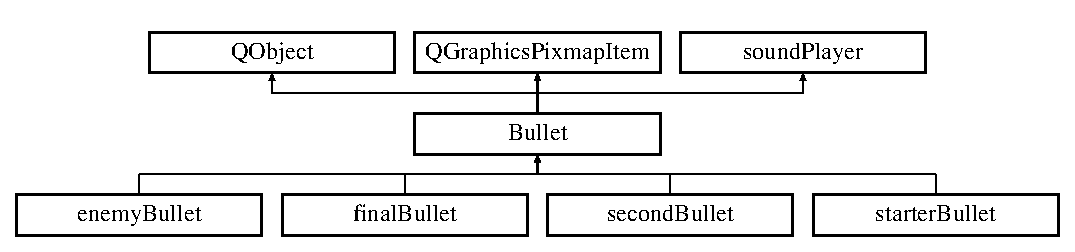
\includegraphics[height=2.937063cm]{classBullet}
\end{center}
\end{figure}
\subsection*{Public Slots}
\begin{DoxyCompactItemize}
\item 
\mbox{\Hypertarget{classBullet_aaeafe4ef62aa04e13e93203a7a9066eb}\label{classBullet_aaeafe4ef62aa04e13e93203a7a9066eb}} 
virtual void \hyperlink{classBullet_aaeafe4ef62aa04e13e93203a7a9066eb}{move} ()=0
\begin{DoxyCompactList}\small\item\em will define the movement in the subclasses \end{DoxyCompactList}\end{DoxyCompactItemize}
\subsection*{Public Member Functions}
\begin{DoxyCompactItemize}
\item 
\mbox{\Hypertarget{classBullet_ae06db7b162490a47736a5e8a61aa2d5f}\label{classBullet_ae06db7b162490a47736a5e8a61aa2d5f}} 
void \hyperlink{classBullet_ae06db7b162490a47736a5e8a61aa2d5f}{play\+Sound} ()
\begin{DoxyCompactList}\small\item\em plays the bullet\+Sound Q\+Media\+Player object with the \hyperlink{classsoundPlayer_a1d187e2c442666b8faa74d07a3694edb}{boom()} function from \hyperlink{classsoundPlayer}{sound\+Player} \end{DoxyCompactList}\item 
\mbox{\Hypertarget{classBullet_a682701fa7f9d4a9564dbcd6ed3f73588}\label{classBullet_a682701fa7f9d4a9564dbcd6ed3f73588}} 
int \hyperlink{classBullet_a682701fa7f9d4a9564dbcd6ed3f73588}{get\+Damage} ()
\begin{DoxyCompactList}\small\item\em Returns the amount of damage that a bullet inflicts. \end{DoxyCompactList}\item 
\mbox{\Hypertarget{classBullet_aaa0132f847fa70a1fcaf165a33e638b1}\label{classBullet_aaa0132f847fa70a1fcaf165a33e638b1}} 
void \hyperlink{classBullet_aaa0132f847fa70a1fcaf165a33e638b1}{set\+Damage} (int arg)
\begin{DoxyCompactList}\small\item\em Sets the amount of damage that a bullet inflcits. \end{DoxyCompactList}\item 
\mbox{\Hypertarget{classBullet_a00ffc9297154f11493f0a664ae2f4f40}\label{classBullet_a00ffc9297154f11493f0a664ae2f4f40}} 
std\+::pair$<$ int, int $>$ \hyperlink{classBullet_a00ffc9297154f11493f0a664ae2f4f40}{get\+Velocity} ()
\begin{DoxyCompactList}\small\item\em Returns the velocity of a bullet. \end{DoxyCompactList}\item 
\mbox{\Hypertarget{classBullet_a9dc2cc1401e02fdb9632ea8fac34cb11}\label{classBullet_a9dc2cc1401e02fdb9632ea8fac34cb11}} 
void \hyperlink{classBullet_a9dc2cc1401e02fdb9632ea8fac34cb11}{set\+Velocity} (std\+::pair$<$ int, int $>$ arg)
\begin{DoxyCompactList}\small\item\em Sets the velocity of a bullet. \end{DoxyCompactList}\item 
\mbox{\Hypertarget{classBullet_a87d32d76ae8f43839013eea1cfc07625}\label{classBullet_a87d32d76ae8f43839013eea1cfc07625}} 
Q\+Media\+Player $\ast$ \hyperlink{classBullet_a87d32d76ae8f43839013eea1cfc07625}{get\+Sound} ()
\begin{DoxyCompactList}\small\item\em Returns a pointer to the Q\+Media\+Player object bullet\+Sound (eg. the variable that plays the bullet\textquotesingle{}s sound) \end{DoxyCompactList}\item 
\mbox{\Hypertarget{classBullet_a07e1aa135f6eafc3c2b1b2938138d1fe}\label{classBullet_a07e1aa135f6eafc3c2b1b2938138d1fe}} 
void \hyperlink{classBullet_a07e1aa135f6eafc3c2b1b2938138d1fe}{set\+Sound} (Q\+Media\+Player $\ast$arg)
\begin{DoxyCompactList}\small\item\em Used to set the bullet\+Sound to the Q\+Media\+Player object that is sent in. \end{DoxyCompactList}\item 
\mbox{\Hypertarget{classBullet_a6266a742a36672d1b023652f3ece4905}\label{classBullet_a6266a742a36672d1b023652f3ece4905}} 
Q\+Timer $\ast$ \hyperlink{classBullet_a6266a742a36672d1b023652f3ece4905}{get\+Timer} ()
\begin{DoxyCompactList}\small\item\em Returns a pointer to the Q\+Media\+Player object timer. \end{DoxyCompactList}\item 
\mbox{\Hypertarget{classBullet_aa1e71a5ffbf610056f80bb54f2cde99f}\label{classBullet_aa1e71a5ffbf610056f80bb54f2cde99f}} 
void \hyperlink{classBullet_aa1e71a5ffbf610056f80bb54f2cde99f}{set\+Timer} (Q\+Timer $\ast$arg)
\begin{DoxyCompactList}\small\item\em Used to set the timer to the Q\+Media\+Player that is sent in. \end{DoxyCompactList}\item 
\mbox{\Hypertarget{classBullet_a2a2d4ad5cca3dddb9eff382d7d1e4a1f}\label{classBullet_a2a2d4ad5cca3dddb9eff382d7d1e4a1f}} 
\hyperlink{structConstants}{Constants} \hyperlink{classBullet_a2a2d4ad5cca3dddb9eff382d7d1e4a1f}{get\+Constants} ()
\begin{DoxyCompactList}\small\item\em Returns the constants of the game. \end{DoxyCompactList}\item 
\mbox{\Hypertarget{classBullet_a394d03770cab61762a5928e54a08174a}\label{classBullet_a394d03770cab61762a5928e54a08174a}} 
bool \hyperlink{classBullet_a394d03770cab61762a5928e54a08174a}{contact} (Q\+List$<$ Q\+Graphics\+Item $\ast$$>$ arg, Q\+Graphics\+Item $\ast$kula)
\begin{DoxyCompactList}\small\item\em Deletes objects that collide with bullets. \end{DoxyCompactList}\end{DoxyCompactItemize}


\subsection{Detailed Description}
\hyperlink{classBullet}{Bullet} base class. 

\hyperlink{classBullet}{Bullet} base class.

Inherits from Q\+Object, Q\+Graphics\+Pix\+Item and \hyperlink{classsoundPlayer}{sound\+Player}. 

The documentation for this class was generated from the following files\+:\begin{DoxyCompactItemize}
\item 
bullet.\+h\item 
bullet.\+cpp\end{DoxyCompactItemize}

\hypertarget{structConstants}{}\section{Constants Struct Reference}
\label{structConstants}\index{Constants@{Constants}}


The \hyperlink{structConstants}{Constants} struct, used to access numbers that are constant throughout the program.  




{\ttfamily \#include $<$constants.\+h$>$}

\subsection*{Public Attributes}
\begin{DoxyCompactItemize}
\item 
\mbox{\Hypertarget{structConstants_ad3d07dd54f58421e5b20f83f6edadf74}\label{structConstants_ad3d07dd54f58421e5b20f83f6edadf74}} 
const size\+\_\+t \hyperlink{structConstants_ad3d07dd54f58421e5b20f83f6edadf74}{W\+I\+D\+TH} = 900
\begin{DoxyCompactList}\small\item\em W\+I\+D\+TH represents the width of the scene. \end{DoxyCompactList}\item 
\mbox{\Hypertarget{structConstants_a0205ca85f89c22f0eccb07001cf4612d}\label{structConstants_a0205ca85f89c22f0eccb07001cf4612d}} 
const size\+\_\+t \hyperlink{structConstants_a0205ca85f89c22f0eccb07001cf4612d}{H\+E\+I\+G\+HT} = 700
\begin{DoxyCompactList}\small\item\em H\+E\+I\+G\+HT represents the height of the scene. \end{DoxyCompactList}\item 
\mbox{\Hypertarget{structConstants_ab58d8adfff12e9aaf322207bf747a6a9}\label{structConstants_ab58d8adfff12e9aaf322207bf747a6a9}} 
const size\+\_\+t \hyperlink{structConstants_ab58d8adfff12e9aaf322207bf747a6a9}{O\+R\+I\+G\+IN} = 0
\begin{DoxyCompactList}\small\item\em O\+R\+I\+G\+IN is used to represent the origin (eg. the point(0, 0)) \end{DoxyCompactList}\item 
\mbox{\Hypertarget{structConstants_ad04c5dd99fb2304ae86ac6a892849a26}\label{structConstants_ad04c5dd99fb2304ae86ac6a892849a26}} 
const size\+\_\+t \hyperlink{structConstants_ad04c5dd99fb2304ae86ac6a892849a26}{first\+Enemy\+Height} = 60
\begin{DoxyCompactList}\small\item\em the height of the \hyperlink{classfirstEnemy}{first\+Enemy} object\textquotesingle{}s photo \end{DoxyCompactList}\item 
\mbox{\Hypertarget{structConstants_a8a5a36685d3c721996d6ba029a1b2c7c}\label{structConstants_a8a5a36685d3c721996d6ba029a1b2c7c}} 
const size\+\_\+t \hyperlink{structConstants_a8a5a36685d3c721996d6ba029a1b2c7c}{first\+Enemy\+Width} = 74
\begin{DoxyCompactList}\small\item\em the width of the \hyperlink{classfirstEnemy}{first\+Enemy} object\textquotesingle{}s photo \end{DoxyCompactList}\item 
\mbox{\Hypertarget{structConstants_a3d86480f3452aa12897b18b321e8760b}\label{structConstants_a3d86480f3452aa12897b18b321e8760b}} 
const size\+\_\+t \hyperlink{structConstants_a3d86480f3452aa12897b18b321e8760b}{second\+Enemy\+Height} = 96
\begin{DoxyCompactList}\small\item\em the height of the \hyperlink{classsecondEnemy}{second\+Enemy} object\textquotesingle{}s photo \end{DoxyCompactList}\item 
\mbox{\Hypertarget{structConstants_a53d023a482ef6ce0aa00d90e83f2e122}\label{structConstants_a53d023a482ef6ce0aa00d90e83f2e122}} 
const size\+\_\+t \hyperlink{structConstants_a53d023a482ef6ce0aa00d90e83f2e122}{second\+Enemy\+Width} = 88
\begin{DoxyCompactList}\small\item\em the width of the \hyperlink{classsecondEnemy}{second\+Enemy} object\textquotesingle{}s photo \end{DoxyCompactList}\item 
\mbox{\Hypertarget{structConstants_a193ec8ce9a3629e1de85bf127c858ae6}\label{structConstants_a193ec8ce9a3629e1de85bf127c858ae6}} 
const size\+\_\+t \hyperlink{structConstants_a193ec8ce9a3629e1de85bf127c858ae6}{final\+Enemy\+Height} = 100
\begin{DoxyCompactList}\small\item\em the height of the \hyperlink{classfinalEnemy}{final\+Enemy} object\textquotesingle{}s photo \end{DoxyCompactList}\item 
\mbox{\Hypertarget{structConstants_acef510139b3ea92c216c3f2d7980a7c1}\label{structConstants_acef510139b3ea92c216c3f2d7980a7c1}} 
const size\+\_\+t \hyperlink{structConstants_acef510139b3ea92c216c3f2d7980a7c1}{final\+Enemy\+Width} = 86
\begin{DoxyCompactList}\small\item\em the width of the \hyperlink{classfinalEnemy}{final\+Enemy} object\textquotesingle{}s photo \end{DoxyCompactList}\item 
\mbox{\Hypertarget{structConstants_af331f72a52cd4c1176970629bedabe31}\label{structConstants_af331f72a52cd4c1176970629bedabe31}} 
const size\+\_\+t \hyperlink{structConstants_af331f72a52cd4c1176970629bedabe31}{enemy\+Bullet\+Size} = 10
\begin{DoxyCompactList}\small\item\em the size of the \hyperlink{classenemyBullet}{enemy\+Bullet} (the \hyperlink{classenemyBullet}{enemy\+Bullet} is the same size in both the x and y axis) \end{DoxyCompactList}\item 
\mbox{\Hypertarget{structConstants_a11f7567f1a874c23c447c7be16e08edc}\label{structConstants_a11f7567f1a874c23c447c7be16e08edc}} 
const size\+\_\+t \hyperlink{structConstants_a11f7567f1a874c23c447c7be16e08edc}{starter\+Bullet\+Size} = 16
\begin{DoxyCompactList}\small\item\em the size of the \hyperlink{classstarterBullet}{starter\+Bullet} (the \hyperlink{classstarterBullet}{starter\+Bullet} is the same size in both the x and the y axis) \end{DoxyCompactList}\item 
\mbox{\Hypertarget{structConstants_a07b9dd1f65aa3f70e09f8f845e867c3a}\label{structConstants_a07b9dd1f65aa3f70e09f8f845e867c3a}} 
const size\+\_\+t \hyperlink{structConstants_a07b9dd1f65aa3f70e09f8f845e867c3a}{second\+Bullet\+Size} = 60
\begin{DoxyCompactList}\small\item\em the size of the \hyperlink{classsecondBullet}{second\+Bullet} \end{DoxyCompactList}\item 
\mbox{\Hypertarget{structConstants_abde3253cd79ffe95316300e006f3115c}\label{structConstants_abde3253cd79ffe95316300e006f3115c}} 
const size\+\_\+t \hyperlink{structConstants_abde3253cd79ffe95316300e006f3115c}{final\+Bullet\+Height} = 130
\begin{DoxyCompactList}\small\item\em the height of the fina\+Bullet \end{DoxyCompactList}\item 
\mbox{\Hypertarget{structConstants_a5f71dc635e410b31e4876e97e46b1c20}\label{structConstants_a5f71dc635e410b31e4876e97e46b1c20}} 
const size\+\_\+t \hyperlink{structConstants_a5f71dc635e410b31e4876e97e46b1c20}{final\+Bullet\+Width} = 115
\begin{DoxyCompactList}\small\item\em the width of the \hyperlink{classfinalBullet}{final\+Bullet} \end{DoxyCompactList}\item 
\mbox{\Hypertarget{structConstants_a9f635dc83697b9a825959384b61cc559}\label{structConstants_a9f635dc83697b9a825959384b61cc559}} 
const size\+\_\+t \hyperlink{structConstants_a9f635dc83697b9a825959384b61cc559}{player\+Height} = 67
\begin{DoxyCompactList}\small\item\em the height of the \hyperlink{classPlayer}{Player} \end{DoxyCompactList}\item 
\mbox{\Hypertarget{structConstants_a9854eedbfb70239ffbd1d12530f301a5}\label{structConstants_a9854eedbfb70239ffbd1d12530f301a5}} 
const size\+\_\+t \hyperlink{structConstants_a9854eedbfb70239ffbd1d12530f301a5}{player\+Width} = 50
\begin{DoxyCompactList}\small\item\em the width of the \hyperlink{classPlayer}{Player} \end{DoxyCompactList}\end{DoxyCompactItemize}


\subsection{Detailed Description}
The \hyperlink{structConstants}{Constants} struct, used to access numbers that are constant throughout the program. 

The documentation for this struct was generated from the following file\+:\begin{DoxyCompactItemize}
\item 
constants.\+h\end{DoxyCompactItemize}

\hypertarget{classEnemy}{}\section{Enemy Class Reference}
\label{classEnemy}\index{Enemy@{Enemy}}


The \hyperlink{classEnemy}{Enemy} class, base class for all enemy objects.  




{\ttfamily \#include $<$enemy.\+h$>$}

Inheritance diagram for Enemy\+:\begin{figure}[H]
\begin{center}
\leavevmode
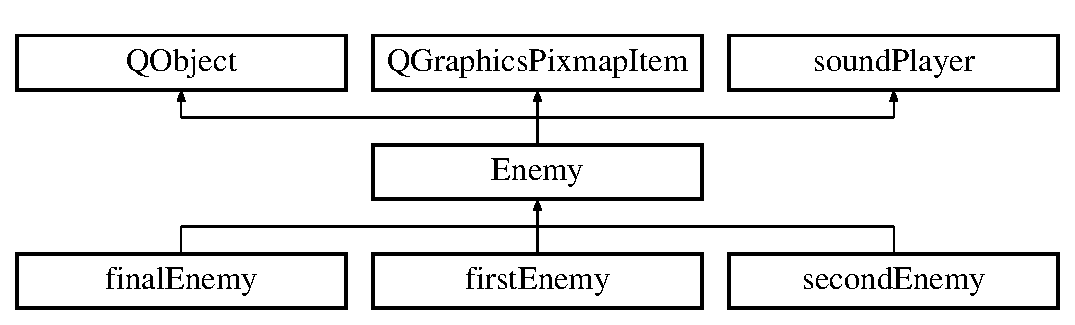
\includegraphics[height=3.000000cm]{classEnemy}
\end{center}
\end{figure}
\subsection*{Public Slots}
\begin{DoxyCompactItemize}
\item 
\mbox{\Hypertarget{classEnemy_a1c208ac4a80b892f9692222bcb96f6ae}\label{classEnemy_a1c208ac4a80b892f9692222bcb96f6ae}} 
virtual void \hyperlink{classEnemy_a1c208ac4a80b892f9692222bcb96f6ae}{move} ()=0
\begin{DoxyCompactList}\small\item\em Will move the enemy object in the subclasses. \end{DoxyCompactList}\item 
\mbox{\Hypertarget{classEnemy_a3208d68423cd0c79d5f2528ebb849dc5}\label{classEnemy_a3208d68423cd0c79d5f2528ebb849dc5}} 
virtual void \hyperlink{classEnemy_a3208d68423cd0c79d5f2528ebb849dc5}{shoot} ()=0
\begin{DoxyCompactList}\small\item\em Will make the enemy shoot a bullet in the subclasses. \end{DoxyCompactList}\end{DoxyCompactItemize}
\subsection*{Public Member Functions}
\begin{DoxyCompactItemize}
\item 
\mbox{\Hypertarget{classEnemy_ad737566e8e9dfb500dd3e177d27cb7f0}\label{classEnemy_ad737566e8e9dfb500dd3e177d27cb7f0}} 
void \hyperlink{classEnemy_ad737566e8e9dfb500dd3e177d27cb7f0}{play\+Sound} (Q\+Media\+Player $\ast$arg)
\begin{DoxyCompactList}\small\item\em Plays the sound that the enemy emits whwn it shoots a bullet. \end{DoxyCompactList}\item 
\mbox{\Hypertarget{classEnemy_a4c66609d3acb845f8cf822e0b47d2c05}\label{classEnemy_a4c66609d3acb845f8cf822e0b47d2c05}} 
std\+::pair$<$ int, int $>$ \hyperlink{classEnemy_a4c66609d3acb845f8cf822e0b47d2c05}{get\+Velocity} ()
\begin{DoxyCompactList}\small\item\em Returns the velocity of the enemy. \end{DoxyCompactList}\item 
\mbox{\Hypertarget{classEnemy_a01b9949a62e439e49cfe95e0ddecb7fe}\label{classEnemy_a01b9949a62e439e49cfe95e0ddecb7fe}} 
void \hyperlink{classEnemy_a01b9949a62e439e49cfe95e0ddecb7fe}{set\+Velocity} (std\+::pair$<$ int, int $>$ arg)
\begin{DoxyCompactList}\small\item\em Sets the velocity of the enemy. \end{DoxyCompactList}\item 
\mbox{\Hypertarget{classEnemy_abe323b8ed67ea623ffb4bab4ff6589e8}\label{classEnemy_abe323b8ed67ea623ffb4bab4ff6589e8}} 
Q\+Timer $\ast$ \hyperlink{classEnemy_abe323b8ed67ea623ffb4bab4ff6589e8}{get\+Timer} ()
\begin{DoxyCompactList}\small\item\em Returns a pointer to the timer. \end{DoxyCompactList}\item 
\mbox{\Hypertarget{classEnemy_ab30ff18d935a67f440bec8d07d48e2e2}\label{classEnemy_ab30ff18d935a67f440bec8d07d48e2e2}} 
void \hyperlink{classEnemy_ab30ff18d935a67f440bec8d07d48e2e2}{set\+Timer} (Q\+Timer $\ast$arg)
\begin{DoxyCompactList}\small\item\em Sets the timer. \end{DoxyCompactList}\item 
\mbox{\Hypertarget{classEnemy_abda21c8dcacf52f59de732d56c7ac012}\label{classEnemy_abda21c8dcacf52f59de732d56c7ac012}} 
Q\+Media\+Player $\ast$ \hyperlink{classEnemy_abda21c8dcacf52f59de732d56c7ac012}{get\+Sound} ()
\begin{DoxyCompactList}\small\item\em Returns a pointer to the Q\+Media\+Player explosion\+Sound. \end{DoxyCompactList}\item 
\mbox{\Hypertarget{classEnemy_a656c43919f972077f20916577594e148}\label{classEnemy_a656c43919f972077f20916577594e148}} 
void \hyperlink{classEnemy_a656c43919f972077f20916577594e148}{set\+Sound} (Q\+Media\+Player $\ast$arg)
\begin{DoxyCompactList}\small\item\em Sets the sound. \end{DoxyCompactList}\item 
\mbox{\Hypertarget{classEnemy_a7d36994bba593bb623e943f9264f901b}\label{classEnemy_a7d36994bba593bb623e943f9264f901b}} 
int \hyperlink{classEnemy_a7d36994bba593bb623e943f9264f901b}{get\+Damage} ()
\begin{DoxyCompactList}\small\item\em Returns the amount of damage that an enemy inflicts. \end{DoxyCompactList}\item 
\mbox{\Hypertarget{classEnemy_ac66eb36302dfb355da9b5b397b165f56}\label{classEnemy_ac66eb36302dfb355da9b5b397b165f56}} 
void \hyperlink{classEnemy_ac66eb36302dfb355da9b5b397b165f56}{set\+Damage} (int \&arg)
\begin{DoxyCompactList}\small\item\em Sets the damage. \end{DoxyCompactList}\item 
\mbox{\Hypertarget{classEnemy_a826bba4cc09bc31cb2512891b797468a}\label{classEnemy_a826bba4cc09bc31cb2512891b797468a}} 
Q\+Timer $\ast$ \hyperlink{classEnemy_a826bba4cc09bc31cb2512891b797468a}{get\+Shooter\+Timer} ()
\begin{DoxyCompactList}\small\item\em Returns a pointer to the Q\+Timer shooter\+Timer. \end{DoxyCompactList}\item 
\mbox{\Hypertarget{classEnemy_ac23a9c502aa5004cb211f0582e876867}\label{classEnemy_ac23a9c502aa5004cb211f0582e876867}} 
void \hyperlink{classEnemy_ac23a9c502aa5004cb211f0582e876867}{set\+Shooter\+Timer} (Q\+Timer $\ast$arg)
\begin{DoxyCompactList}\small\item\em Set the Q\+Timer shooter\+Timer. \end{DoxyCompactList}\item 
\mbox{\Hypertarget{classEnemy_af0f8e420ba12100a2069647b0992e4cf}\label{classEnemy_af0f8e420ba12100a2069647b0992e4cf}} 
\hyperlink{structConstants}{Constants} \hyperlink{classEnemy_af0f8e420ba12100a2069647b0992e4cf}{get\+Constants} ()
\begin{DoxyCompactList}\small\item\em Returns the constants. \end{DoxyCompactList}\end{DoxyCompactItemize}


\subsection{Detailed Description}
The \hyperlink{classEnemy}{Enemy} class, base class for all enemy objects. 

The documentation for this class was generated from the following file\+:\begin{DoxyCompactItemize}
\item 
enemy.\+h\end{DoxyCompactItemize}

\hypertarget{classenemyBullet}{}\section{enemy\+Bullet Class Reference}
\label{classenemyBullet}\index{enemy\+Bullet@{enemy\+Bullet}}


The \hyperlink{classenemyBullet}{enemy\+Bullet} class, inherits from the baseclass \hyperlink{classBullet}{Bullet}.  




{\ttfamily \#include $<$enemybullet.\+h$>$}

Inheritance diagram for enemy\+Bullet\+:\begin{figure}[H]
\begin{center}
\leavevmode
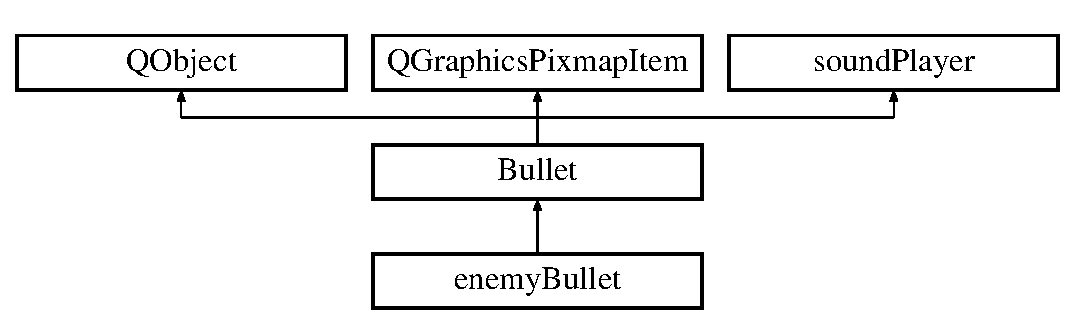
\includegraphics[height=3.000000cm]{classenemyBullet}
\end{center}
\end{figure}
\subsection*{Public Member Functions}
\begin{DoxyCompactItemize}
\item 
bool \hyperlink{classenemyBullet_a2e2e8de44bed2bff6b949b39a61efba9}{player\+Contact} (Q\+List$<$ Q\+Graphics\+Item $\ast$$>$ arg, \hyperlink{classenemyBullet}{enemy\+Bullet} $\ast$kula)
\begin{DoxyCompactList}\small\item\em When a bullet hits the player. \end{DoxyCompactList}\end{DoxyCompactItemize}
\subsection*{Additional Inherited Members}


\subsection{Detailed Description}
The \hyperlink{classenemyBullet}{enemy\+Bullet} class, inherits from the baseclass \hyperlink{classBullet}{Bullet}. 

\subsection{Member Function Documentation}
\mbox{\Hypertarget{classenemyBullet_a2e2e8de44bed2bff6b949b39a61efba9}\label{classenemyBullet_a2e2e8de44bed2bff6b949b39a61efba9}} 
\index{enemy\+Bullet@{enemy\+Bullet}!player\+Contact@{player\+Contact}}
\index{player\+Contact@{player\+Contact}!enemy\+Bullet@{enemy\+Bullet}}
\subsubsection{\texorpdfstring{player\+Contact()}{playerContact()}}
{\footnotesize\ttfamily bool enemy\+Bullet\+::player\+Contact (\begin{DoxyParamCaption}\item[{Q\+List$<$ Q\+Graphics\+Item $\ast$$>$}]{arg,  }\item[{\hyperlink{classenemyBullet}{enemy\+Bullet} $\ast$}]{kula }\end{DoxyParamCaption})}



When a bullet hits the player. 

player\+Contact 
\begin{DoxyParams}{Parameters}
{\em arg} & \\
\hline
{\em kula} & \\
\hline
\end{DoxyParams}
\begin{DoxyReturn}{Returns}
True if the player has been hit, False if not
\end{DoxyReturn}
Traverse the Q\+List (arg) of colliding\+Items If the player has been hit, decrease the players health. 

The documentation for this class was generated from the following files\+:\begin{DoxyCompactItemize}
\item 
enemybullet.\+h\item 
enemybullet.\+cpp\end{DoxyCompactItemize}

\hypertarget{classfinalBullet}{}\section{final\+Bullet Class Reference}
\label{classfinalBullet}\index{final\+Bullet@{final\+Bullet}}


The \hyperlink{classfinalBullet}{final\+Bullet} class, inherits from the baseclass \hyperlink{classBullet}{Bullet}.  




{\ttfamily \#include $<$finalbullet.\+h$>$}

Inheritance diagram for final\+Bullet\+:\begin{figure}[H]
\begin{center}
\leavevmode
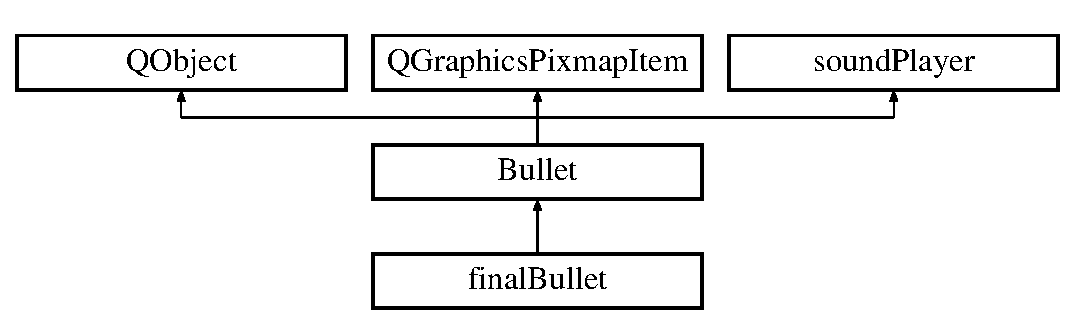
\includegraphics[height=3.000000cm]{classfinalBullet}
\end{center}
\end{figure}
\subsection*{Public Slots}
\begin{DoxyCompactItemize}
\item 
\mbox{\Hypertarget{classfinalBullet_aae61a14632d24b5dfc5ceec785b1d94b}\label{classfinalBullet_aae61a14632d24b5dfc5ceec785b1d94b}} 
void \hyperlink{classfinalBullet_aae61a14632d24b5dfc5ceec785b1d94b}{move} ()
\begin{DoxyCompactList}\small\item\em moves the bullet \end{DoxyCompactList}\end{DoxyCompactItemize}
\subsection*{Public Member Functions}
\begin{DoxyCompactItemize}
\item 
\mbox{\Hypertarget{classfinalBullet_aef126a4c178fe484b1766a2584ff3096}\label{classfinalBullet_aef126a4c178fe484b1766a2584ff3096}} 
\hyperlink{classfinalBullet_aef126a4c178fe484b1766a2584ff3096}{final\+Bullet} ()
\begin{DoxyCompactList}\small\item\em constructor \end{DoxyCompactList}\end{DoxyCompactItemize}


\subsection{Detailed Description}
The \hyperlink{classfinalBullet}{final\+Bullet} class, inherits from the baseclass \hyperlink{classBullet}{Bullet}. 

The documentation for this class was generated from the following files\+:\begin{DoxyCompactItemize}
\item 
finalbullet.\+h\item 
finalbullet.\+cpp\end{DoxyCompactItemize}

\hypertarget{classfinalEnemy}{}\section{final\+Enemy Class Reference}
\label{classfinalEnemy}\index{final\+Enemy@{final\+Enemy}}


The \hyperlink{classfinalEnemy}{final\+Enemy} class, inherits from the baseclass \hyperlink{classEnemy}{Enemy}.  




{\ttfamily \#include $<$finalenemy.\+h$>$}

Inheritance diagram for final\+Enemy\+:\begin{figure}[H]
\begin{center}
\leavevmode
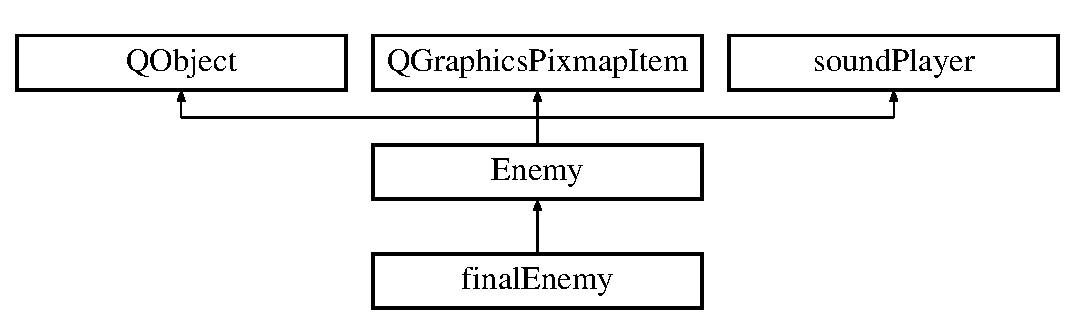
\includegraphics[height=3.000000cm]{classfinalEnemy}
\end{center}
\end{figure}
\subsection*{Public Slots}
\begin{DoxyCompactItemize}
\item 
\mbox{\Hypertarget{classfinalEnemy_a9422198ed38d374edff347744cae7f9d}\label{classfinalEnemy_a9422198ed38d374edff347744cae7f9d}} 
void \hyperlink{classfinalEnemy_a9422198ed38d374edff347744cae7f9d}{move} ()
\begin{DoxyCompactList}\small\item\em moves the enemy \end{DoxyCompactList}\item 
\mbox{\Hypertarget{classfinalEnemy_a525be5392591999ed81d67145a68374c}\label{classfinalEnemy_a525be5392591999ed81d67145a68374c}} 
void \hyperlink{classfinalEnemy_a525be5392591999ed81d67145a68374c}{shoot} ()
\begin{DoxyCompactList}\small\item\em when the enemy shoots, this function is invoked \end{DoxyCompactList}\end{DoxyCompactItemize}
\subsection*{Public Member Functions}
\begin{DoxyCompactItemize}
\item 
\mbox{\Hypertarget{classfinalEnemy_ad8c93e80b7f2ca279a777bed6d209401}\label{classfinalEnemy_ad8c93e80b7f2ca279a777bed6d209401}} 
\hyperlink{classfinalEnemy_ad8c93e80b7f2ca279a777bed6d209401}{final\+Enemy} ()
\begin{DoxyCompactList}\small\item\em constructor \end{DoxyCompactList}\end{DoxyCompactItemize}


\subsection{Detailed Description}
The \hyperlink{classfinalEnemy}{final\+Enemy} class, inherits from the baseclass \hyperlink{classEnemy}{Enemy}. 

The documentation for this class was generated from the following files\+:\begin{DoxyCompactItemize}
\item 
finalenemy.\+h\item 
finalenemy.\+cpp\end{DoxyCompactItemize}

\hypertarget{classfirstEnemy}{}\section{first\+Enemy Class Reference}
\label{classfirstEnemy}\index{first\+Enemy@{first\+Enemy}}


The \hyperlink{classfirstEnemy}{first\+Enemy} class, inherits from the baseclass \hyperlink{classEnemy}{Enemy}.  




{\ttfamily \#include $<$firstenemy.\+h$>$}

Inheritance diagram for first\+Enemy\+:\begin{figure}[H]
\begin{center}
\leavevmode
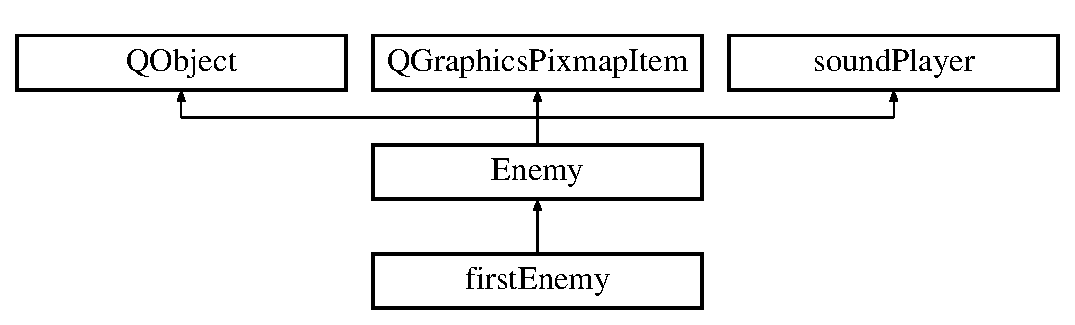
\includegraphics[height=3.000000cm]{classfirstEnemy}
\end{center}
\end{figure}
\subsection*{Public Slots}
\begin{DoxyCompactItemize}
\item 
\mbox{\Hypertarget{classfirstEnemy_acfbe192460fb5c355fd16b7defb20076}\label{classfirstEnemy_acfbe192460fb5c355fd16b7defb20076}} 
void \hyperlink{classfirstEnemy_acfbe192460fb5c355fd16b7defb20076}{move} ()
\begin{DoxyCompactList}\small\item\em moves the enemy \end{DoxyCompactList}\item 
\mbox{\Hypertarget{classfirstEnemy_abb18fa8de737346a07c7c2772edd098c}\label{classfirstEnemy_abb18fa8de737346a07c7c2772edd098c}} 
void \hyperlink{classfirstEnemy_abb18fa8de737346a07c7c2772edd098c}{shoot} ()
\begin{DoxyCompactList}\small\item\em wen the enemy shoots this function is invoked \end{DoxyCompactList}\end{DoxyCompactItemize}
\subsection*{Public Member Functions}
\begin{DoxyCompactItemize}
\item 
\mbox{\Hypertarget{classfirstEnemy_af56c2b9a8dfc696a6f43c171e860e1fd}\label{classfirstEnemy_af56c2b9a8dfc696a6f43c171e860e1fd}} 
\hyperlink{classfirstEnemy_af56c2b9a8dfc696a6f43c171e860e1fd}{first\+Enemy} ()
\begin{DoxyCompactList}\small\item\em constructor \end{DoxyCompactList}\item 
\mbox{\Hypertarget{classfirstEnemy_a25f54a3161da80321f6f9f2c713f83e3}\label{classfirstEnemy_a25f54a3161da80321f6f9f2c713f83e3}} 
\hyperlink{classfirstEnemy_a25f54a3161da80321f6f9f2c713f83e3}{$\sim$first\+Enemy} ()
\begin{DoxyCompactList}\small\item\em destructor \end{DoxyCompactList}\end{DoxyCompactItemize}


\subsection{Detailed Description}
The \hyperlink{classfirstEnemy}{first\+Enemy} class, inherits from the baseclass \hyperlink{classEnemy}{Enemy}. 

The documentation for this class was generated from the following files\+:\begin{DoxyCompactItemize}
\item 
firstenemy.\+h\item 
firstenemy.\+cpp\end{DoxyCompactItemize}

\hypertarget{classGame}{}\section{Game Class Reference}
\label{classGame}\index{Game@{Game}}


The \hyperlink{classGame}{Game} class, used to handle the game logic.  




{\ttfamily \#include $<$game.\+h$>$}

Inheritance diagram for Game\+:\begin{figure}[H]
\begin{center}
\leavevmode
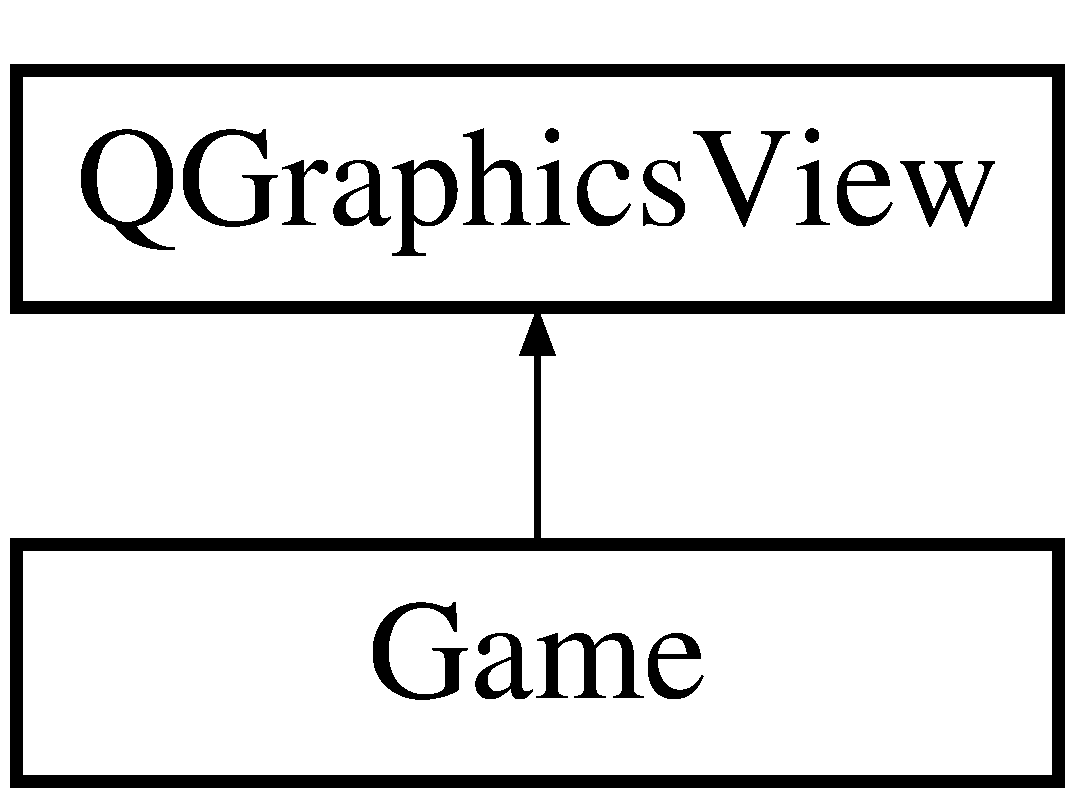
\includegraphics[height=2.000000cm]{classGame}
\end{center}
\end{figure}
\subsection*{Public Member Functions}
\begin{DoxyCompactItemize}
\item 
\mbox{\Hypertarget{classGame_ad59df6562a58a614fda24622d3715b65}\label{classGame_ad59df6562a58a614fda24622d3715b65}} 
\hyperlink{classGame_ad59df6562a58a614fda24622d3715b65}{Game} ()
\begin{DoxyCompactList}\small\item\em Constructor. \end{DoxyCompactList}\item 
\mbox{\Hypertarget{classGame_a0628da809900ad86c1f1968fef3ae620}\label{classGame_a0628da809900ad86c1f1968fef3ae620}} 
\hyperlink{classHealth}{Health} $\ast$ \hyperlink{classGame_a0628da809900ad86c1f1968fef3ae620}{get\+Health} ()
\begin{DoxyCompactList}\small\item\em Retruns the \hyperlink{classHealth}{Health} Q\+Graphics\+Text\+Item. \end{DoxyCompactList}\item 
\mbox{\Hypertarget{classGame_a639ba22fbc6153691a046d18dfe27f3c}\label{classGame_a639ba22fbc6153691a046d18dfe27f3c}} 
\hyperlink{classScore}{Score} $\ast$ \hyperlink{classGame_a639ba22fbc6153691a046d18dfe27f3c}{get\+Score} ()
\begin{DoxyCompactList}\small\item\em Returns the \hyperlink{classScore}{Score} Q\+Graphics\+Text\+Item. \end{DoxyCompactList}\item 
\mbox{\Hypertarget{classGame_a53141ff044e4aa43f23d7dbed11272f6}\label{classGame_a53141ff044e4aa43f23d7dbed11272f6}} 
int \hyperlink{classGame_a53141ff044e4aa43f23d7dbed11272f6}{get\+Level} ()
\begin{DoxyCompactList}\small\item\em returns the current level \end{DoxyCompactList}\item 
\mbox{\Hypertarget{classGame_a6ddcd758ee17faece0f59b691ee57457}\label{classGame_a6ddcd758ee17faece0f59b691ee57457}} 
void \hyperlink{classGame_a6ddcd758ee17faece0f59b691ee57457}{set\+Level} (int arg)
\begin{DoxyCompactList}\small\item\em Sets the level. \end{DoxyCompactList}\item 
\mbox{\Hypertarget{classGame_ac7d371f3f30513a4f3c57f521fac9b5f}\label{classGame_ac7d371f3f30513a4f3c57f521fac9b5f}} 
void \hyperlink{classGame_ac7d371f3f30513a4f3c57f521fac9b5f}{game\+Over} ()
\begin{DoxyCompactList}\small\item\em when the player health passes zero this function is invoked \end{DoxyCompactList}\end{DoxyCompactItemize}


\subsection{Detailed Description}
The \hyperlink{classGame}{Game} class, used to handle the game logic. 

The documentation for this class was generated from the following files\+:\begin{DoxyCompactItemize}
\item 
game.\+h\item 
game.\+cpp\end{DoxyCompactItemize}

\hypertarget{classHealth}{}\section{Health Class Reference}
\label{classHealth}\index{Health@{Health}}


The \hyperlink{classHealth}{Health} class, inherits from Q\+Graphics\+Text\+Item.  




{\ttfamily \#include $<$health.\+h$>$}

Inheritance diagram for Health\+:\begin{figure}[H]
\begin{center}
\leavevmode
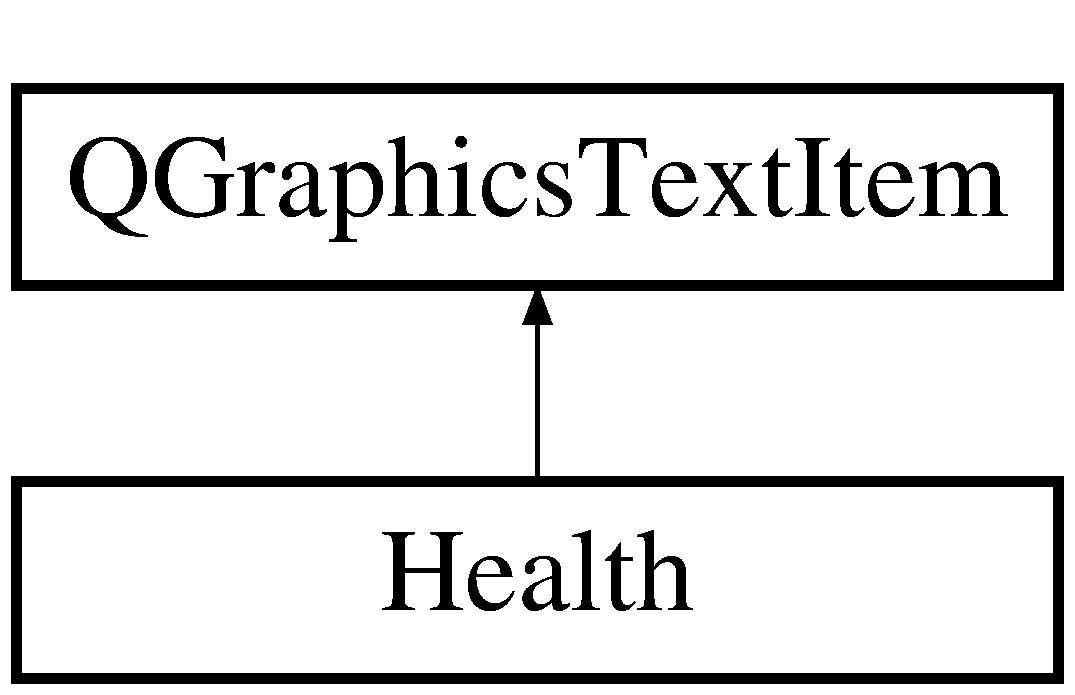
\includegraphics[height=2.000000cm]{classHealth}
\end{center}
\end{figure}
\subsection*{Public Member Functions}
\begin{DoxyCompactItemize}
\item 
\mbox{\Hypertarget{classHealth_a942d89536a25defa8bbac43174cf349c}\label{classHealth_a942d89536a25defa8bbac43174cf349c}} 
\hyperlink{classHealth_a942d89536a25defa8bbac43174cf349c}{Health} (Q\+Graphics\+Text\+Item $\ast$parent=0)
\begin{DoxyCompactList}\small\item\em constructor \end{DoxyCompactList}\item 
\mbox{\Hypertarget{classHealth_adc5f045b9f6937c592e196821d7a6878}\label{classHealth_adc5f045b9f6937c592e196821d7a6878}} 
int \hyperlink{classHealth_adc5f045b9f6937c592e196821d7a6878}{get\+Health} ()
\begin{DoxyCompactList}\small\item\em returns the amount of health the player has \end{DoxyCompactList}\item 
\mbox{\Hypertarget{classHealth_af7d311e68d9214d3479774d9b8e3aaf4}\label{classHealth_af7d311e68d9214d3479774d9b8e3aaf4}} 
void \hyperlink{classHealth_af7d311e68d9214d3479774d9b8e3aaf4}{decrease} (int arg)
\begin{DoxyCompactList}\small\item\em decreases the player helath \end{DoxyCompactList}\item 
\mbox{\Hypertarget{classHealth_a08c580a1587c46316e39b766e4e06fb8}\label{classHealth_a08c580a1587c46316e39b766e4e06fb8}} 
void \hyperlink{classHealth_a08c580a1587c46316e39b766e4e06fb8}{refresh\+Health} ()
\begin{DoxyCompactList}\small\item\em refreshes the screen when the amount of health is changed \end{DoxyCompactList}\end{DoxyCompactItemize}


\subsection{Detailed Description}
The \hyperlink{classHealth}{Health} class, inherits from Q\+Graphics\+Text\+Item. 

The documentation for this class was generated from the following files\+:\begin{DoxyCompactItemize}
\item 
health.\+h\item 
health.\+cpp\end{DoxyCompactItemize}

\hypertarget{classPlayer}{}\section{Player Class Reference}
\label{classPlayer}\index{Player@{Player}}


The \hyperlink{classPlayer}{Player} class, handles player logic and is used to spawn enemies.  




{\ttfamily \#include $<$player.\+h$>$}

Inheritance diagram for Player\+:\begin{figure}[H]
\begin{center}
\leavevmode
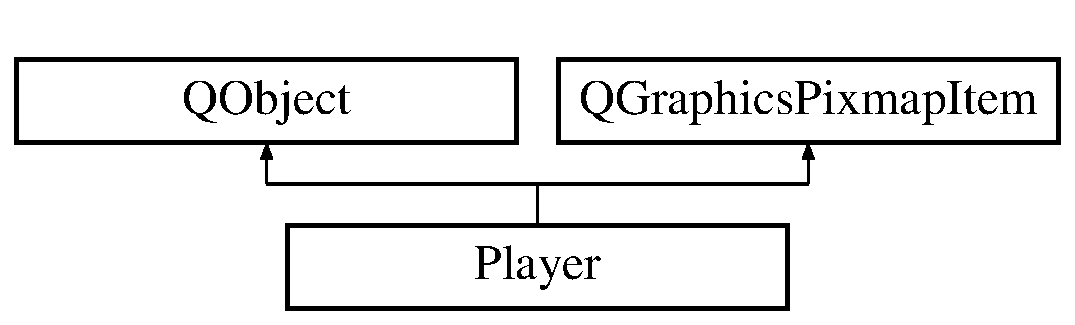
\includegraphics[height=2.000000cm]{classPlayer}
\end{center}
\end{figure}
\subsection*{Public Slots}
\begin{DoxyCompactItemize}
\item 
\mbox{\Hypertarget{classPlayer_a60c45a096af43067179eb8c805e1e76d}\label{classPlayer_a60c45a096af43067179eb8c805e1e76d}} 
void \hyperlink{classPlayer_a60c45a096af43067179eb8c805e1e76d}{move\+Player} ()
\begin{DoxyCompactList}\small\item\em moves the player \end{DoxyCompactList}\item 
\mbox{\Hypertarget{classPlayer_a59ae3f2c7151032a85e58b1591cad769}\label{classPlayer_a59ae3f2c7151032a85e58b1591cad769}} 
void \hyperlink{classPlayer_a59ae3f2c7151032a85e58b1591cad769}{spawn} ()
\begin{DoxyCompactList}\small\item\em spawns enemys \end{DoxyCompactList}\item 
\mbox{\Hypertarget{classPlayer_aa7a25ab9a055e6483c5af1940ce28b74}\label{classPlayer_aa7a25ab9a055e6483c5af1940ce28b74}} 
void \hyperlink{classPlayer_aa7a25ab9a055e6483c5af1940ce28b74}{check\+Score} ()
\begin{DoxyCompactList}\small\item\em checks the score, increases the level when points are high enough \end{DoxyCompactList}\item 
\mbox{\Hypertarget{classPlayer_a615de784bd638d443df5d828535d4018}\label{classPlayer_a615de784bd638d443df5d828535d4018}} 
void \hyperlink{classPlayer_a615de784bd638d443df5d828535d4018}{check\+Health} ()
\begin{DoxyCompactList}\small\item\em Checks the player health. \end{DoxyCompactList}\end{DoxyCompactItemize}
\subsection*{Public Member Functions}
\begin{DoxyCompactItemize}
\item 
\mbox{\Hypertarget{classPlayer_aa3689d20c55d7dfe735cf47c2d6d7dbb}\label{classPlayer_aa3689d20c55d7dfe735cf47c2d6d7dbb}} 
\hyperlink{classPlayer_aa3689d20c55d7dfe735cf47c2d6d7dbb}{Player} (Q\+Graphics\+Pixmap\+Item $\ast$parent=0)
\begin{DoxyCompactList}\small\item\em Constructor. \end{DoxyCompactList}\item 
void \hyperlink{classPlayer_a4d269c4118c29b0ee85c1e0f674260ee}{key\+Press\+Event} (Q\+Key\+Event $\ast$event)
\end{DoxyCompactItemize}


\subsection{Detailed Description}
The \hyperlink{classPlayer}{Player} class, handles player logic and is used to spawn enemies. 

\subsection{Member Function Documentation}
\mbox{\Hypertarget{classPlayer_a4d269c4118c29b0ee85c1e0f674260ee}\label{classPlayer_a4d269c4118c29b0ee85c1e0f674260ee}} 
\index{Player@{Player}!key\+Press\+Event@{key\+Press\+Event}}
\index{key\+Press\+Event@{key\+Press\+Event}!Player@{Player}}
\subsubsection{\texorpdfstring{key\+Press\+Event()}{keyPressEvent()}}
{\footnotesize\ttfamily void Player\+::key\+Press\+Event (\begin{DoxyParamCaption}\item[{Q\+Key\+Event $\ast$}]{event }\end{DoxyParamCaption})}

key\+Press\+Event Used to take input form the player 

The documentation for this class was generated from the following files\+:\begin{DoxyCompactItemize}
\item 
player.\+h\item 
player.\+cpp\end{DoxyCompactItemize}

\hypertarget{classScore}{}\section{Score Class Reference}
\label{classScore}\index{Score@{Score}}


The \hyperlink{classScore}{Score} class, inherits from Q\+Graphics\+Text\+Item.  




{\ttfamily \#include $<$score.\+h$>$}

Inheritance diagram for Score\+:\begin{figure}[H]
\begin{center}
\leavevmode
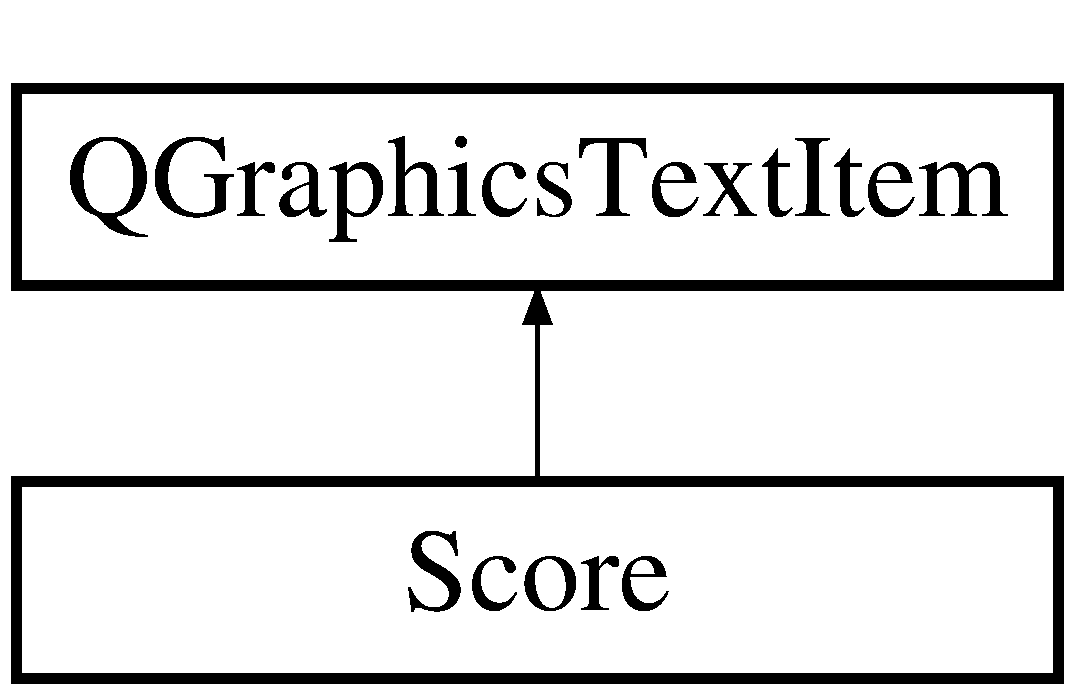
\includegraphics[height=2.000000cm]{classScore}
\end{center}
\end{figure}
\subsection*{Public Member Functions}
\begin{DoxyCompactItemize}
\item 
\mbox{\Hypertarget{classScore_aa80a5a37ab48264a8862849c9d72b740}\label{classScore_aa80a5a37ab48264a8862849c9d72b740}} 
\hyperlink{classScore_aa80a5a37ab48264a8862849c9d72b740}{Score} (Q\+Graphics\+Text\+Item $\ast$parent=0)
\begin{DoxyCompactList}\small\item\em constructor \end{DoxyCompactList}\item 
\mbox{\Hypertarget{classScore_a9a580e858558c0a02cfbd21a19e0a6e2}\label{classScore_a9a580e858558c0a02cfbd21a19e0a6e2}} 
void \hyperlink{classScore_a9a580e858558c0a02cfbd21a19e0a6e2}{increase} (int arg)
\begin{DoxyCompactList}\small\item\em increases the player score \end{DoxyCompactList}\item 
\mbox{\Hypertarget{classScore_a8627c93270c188a3fd28a25b1d07a9e7}\label{classScore_a8627c93270c188a3fd28a25b1d07a9e7}} 
int \hyperlink{classScore_a8627c93270c188a3fd28a25b1d07a9e7}{get\+Score} ()
\begin{DoxyCompactList}\small\item\em returns the player score \end{DoxyCompactList}\item 
\mbox{\Hypertarget{classScore_a2770723408a4db5cdf42b17528bcd460}\label{classScore_a2770723408a4db5cdf42b17528bcd460}} 
void \hyperlink{classScore_a2770723408a4db5cdf42b17528bcd460}{refresh\+Score} ()
\begin{DoxyCompactList}\small\item\em refreshes the score when the score is changed \end{DoxyCompactList}\end{DoxyCompactItemize}


\subsection{Detailed Description}
The \hyperlink{classScore}{Score} class, inherits from Q\+Graphics\+Text\+Item. 

The documentation for this class was generated from the following files\+:\begin{DoxyCompactItemize}
\item 
score.\+h\item 
score.\+cpp\end{DoxyCompactItemize}

\hypertarget{classsecondBullet}{}\section{second\+Bullet Class Reference}
\label{classsecondBullet}\index{second\+Bullet@{second\+Bullet}}


The \hyperlink{classsecondBullet}{second\+Bullet} class, inherits from the baseclass \hyperlink{classBullet}{Bullet}.  




{\ttfamily \#include $<$secondbullet.\+h$>$}

Inheritance diagram for second\+Bullet\+:\begin{figure}[H]
\begin{center}
\leavevmode
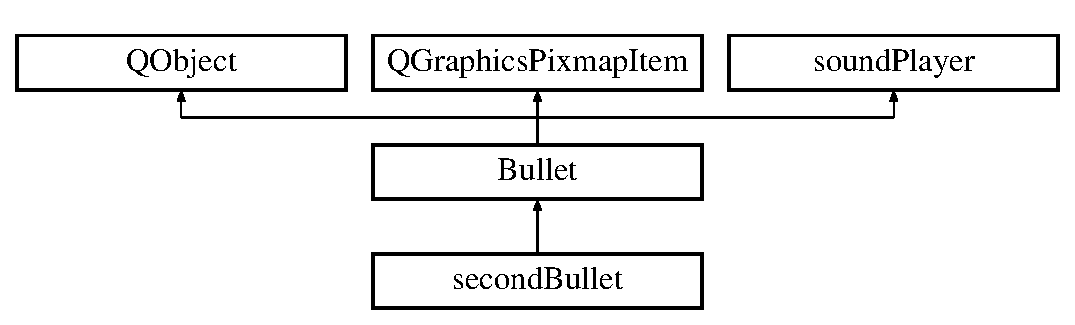
\includegraphics[height=3.000000cm]{classsecondBullet}
\end{center}
\end{figure}
\subsection*{Public Slots}
\begin{DoxyCompactItemize}
\item 
\mbox{\Hypertarget{classsecondBullet_a81df90840307b5ec6d28a9559ce5335d}\label{classsecondBullet_a81df90840307b5ec6d28a9559ce5335d}} 
void \hyperlink{classsecondBullet_a81df90840307b5ec6d28a9559ce5335d}{move} ()
\begin{DoxyCompactList}\small\item\em moves the bullet \end{DoxyCompactList}\end{DoxyCompactItemize}
\subsection*{Public Member Functions}
\begin{DoxyCompactItemize}
\item 
\mbox{\Hypertarget{classsecondBullet_a10822241539609e1a25f5dcae583b96b}\label{classsecondBullet_a10822241539609e1a25f5dcae583b96b}} 
\hyperlink{classsecondBullet_a10822241539609e1a25f5dcae583b96b}{second\+Bullet} ()
\begin{DoxyCompactList}\small\item\em constructor \end{DoxyCompactList}\end{DoxyCompactItemize}


\subsection{Detailed Description}
The \hyperlink{classsecondBullet}{second\+Bullet} class, inherits from the baseclass \hyperlink{classBullet}{Bullet}. 

The documentation for this class was generated from the following files\+:\begin{DoxyCompactItemize}
\item 
secondbullet.\+h\item 
secondbullet.\+cpp\end{DoxyCompactItemize}

\hypertarget{classsecondEnemy}{}\section{second\+Enemy Class Reference}
\label{classsecondEnemy}\index{second\+Enemy@{second\+Enemy}}


The \hyperlink{classsecondEnemy}{second\+Enemy} class, inherits from the baseclass \hyperlink{classEnemy}{Enemy}.  




{\ttfamily \#include $<$secondenemy.\+h$>$}

Inheritance diagram for second\+Enemy\+:\begin{figure}[H]
\begin{center}
\leavevmode
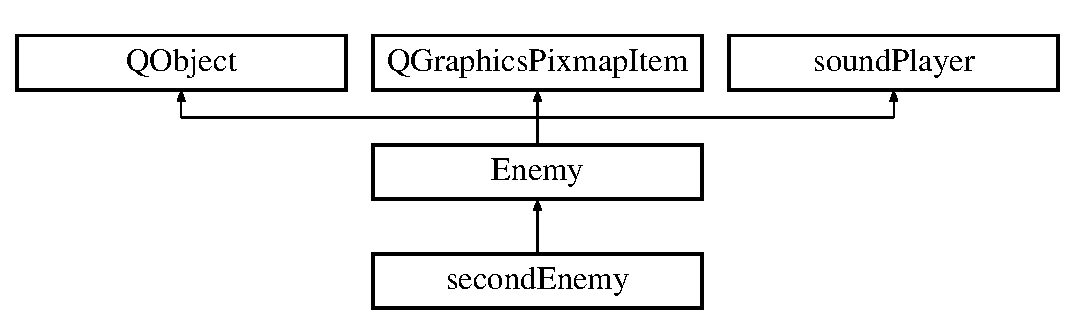
\includegraphics[height=3.000000cm]{classsecondEnemy}
\end{center}
\end{figure}
\subsection*{Public Slots}
\begin{DoxyCompactItemize}
\item 
\mbox{\Hypertarget{classsecondEnemy_a08d9487c6e04c4e7da2ba1353c000de8}\label{classsecondEnemy_a08d9487c6e04c4e7da2ba1353c000de8}} 
void \hyperlink{classsecondEnemy_a08d9487c6e04c4e7da2ba1353c000de8}{move} ()
\begin{DoxyCompactList}\small\item\em moves the enemy \end{DoxyCompactList}\item 
\mbox{\Hypertarget{classsecondEnemy_a592a963fc521a4073acfb3d320179383}\label{classsecondEnemy_a592a963fc521a4073acfb3d320179383}} 
void \hyperlink{classsecondEnemy_a592a963fc521a4073acfb3d320179383}{shoot} ()
\begin{DoxyCompactList}\small\item\em when the enemy shoots this function is invoked \end{DoxyCompactList}\end{DoxyCompactItemize}
\subsection*{Public Member Functions}
\begin{DoxyCompactItemize}
\item 
\mbox{\Hypertarget{classsecondEnemy_a13a43a786499033936a67a31f616443c}\label{classsecondEnemy_a13a43a786499033936a67a31f616443c}} 
\hyperlink{classsecondEnemy_a13a43a786499033936a67a31f616443c}{second\+Enemy} ()
\begin{DoxyCompactList}\small\item\em constructor \end{DoxyCompactList}\item 
\mbox{\Hypertarget{classsecondEnemy_a07f1047b76368ca83f0b4eebc33b31ba}\label{classsecondEnemy_a07f1047b76368ca83f0b4eebc33b31ba}} 
\hyperlink{classsecondEnemy_a07f1047b76368ca83f0b4eebc33b31ba}{$\sim$second\+Enemy} ()
\begin{DoxyCompactList}\small\item\em destructor \end{DoxyCompactList}\end{DoxyCompactItemize}


\subsection{Detailed Description}
The \hyperlink{classsecondEnemy}{second\+Enemy} class, inherits from the baseclass \hyperlink{classEnemy}{Enemy}. 

The documentation for this class was generated from the following files\+:\begin{DoxyCompactItemize}
\item 
secondenemy.\+h\item 
secondenemy.\+cpp\end{DoxyCompactItemize}

\hypertarget{classsoundPlayer}{}\section{sound\+Player Class Reference}
\label{classsoundPlayer}\index{sound\+Player@{sound\+Player}}


The \hyperlink{classsoundPlayer}{sound\+Player} class, used to play sounds.  




{\ttfamily \#include $<$soundplayer.\+h$>$}

Inheritance diagram for sound\+Player\+:\begin{figure}[H]
\begin{center}
\leavevmode
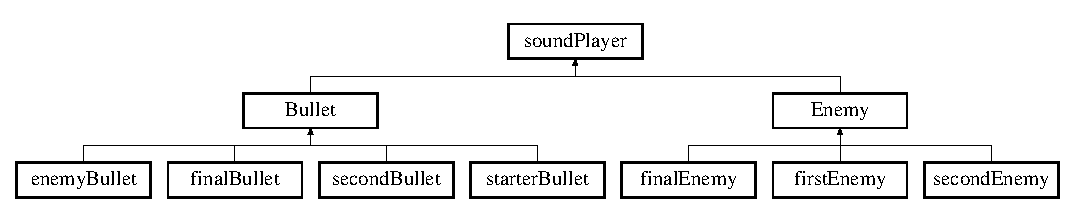
\includegraphics[height=2.424242cm]{classsoundPlayer}
\end{center}
\end{figure}
\subsection*{Public Member Functions}
\begin{DoxyCompactItemize}
\item 
\mbox{\Hypertarget{classsoundPlayer_a1d187e2c442666b8faa74d07a3694edb}\label{classsoundPlayer_a1d187e2c442666b8faa74d07a3694edb}} 
void \hyperlink{classsoundPlayer_a1d187e2c442666b8faa74d07a3694edb}{boom} (Q\+Media\+Player $\ast$arg)
\begin{DoxyCompactList}\small\item\em boom function, takes a Q\+Media\+Player pointer as an argument and plays it\textquotesingle{}s sound \end{DoxyCompactList}\end{DoxyCompactItemize}


\subsection{Detailed Description}
The \hyperlink{classsoundPlayer}{sound\+Player} class, used to play sounds. 

The documentation for this class was generated from the following file\+:\begin{DoxyCompactItemize}
\item 
soundplayer.\+h\end{DoxyCompactItemize}

\hypertarget{classstarterBullet}{}\section{starter\+Bullet Class Reference}
\label{classstarterBullet}\index{starter\+Bullet@{starter\+Bullet}}


The \hyperlink{classstarterBullet}{starter\+Bullet} class, inherits from the baseclass \hyperlink{classBullet}{Bullet}.  




{\ttfamily \#include $<$starterbullet.\+h$>$}

Inheritance diagram for starter\+Bullet\+:\begin{figure}[H]
\begin{center}
\leavevmode
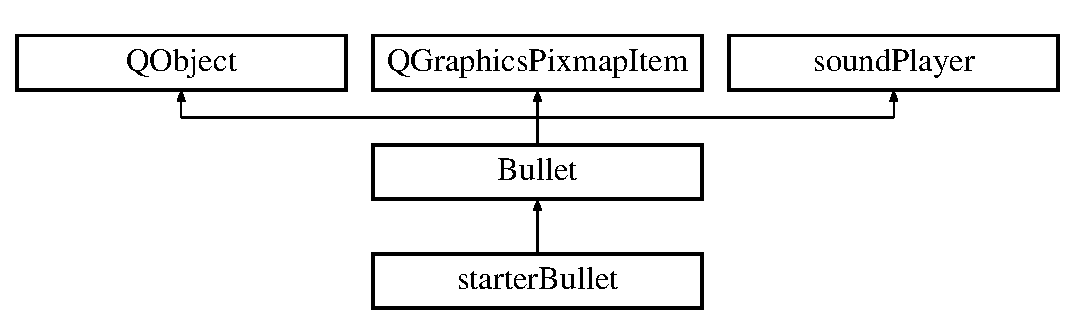
\includegraphics[height=3.000000cm]{classstarterBullet}
\end{center}
\end{figure}
\subsection*{Public Slots}
\begin{DoxyCompactItemize}
\item 
\mbox{\Hypertarget{classstarterBullet_a24f547b4b243d174013d9b231a07e85c}\label{classstarterBullet_a24f547b4b243d174013d9b231a07e85c}} 
void \hyperlink{classstarterBullet_a24f547b4b243d174013d9b231a07e85c}{move} ()
\begin{DoxyCompactList}\small\item\em moves the bullet \end{DoxyCompactList}\end{DoxyCompactItemize}
\subsection*{Public Member Functions}
\begin{DoxyCompactItemize}
\item 
\mbox{\Hypertarget{classstarterBullet_a62bf9e24bb38f03b4adea5590b1e0a87}\label{classstarterBullet_a62bf9e24bb38f03b4adea5590b1e0a87}} 
\hyperlink{classstarterBullet_a62bf9e24bb38f03b4adea5590b1e0a87}{starter\+Bullet} ()
\begin{DoxyCompactList}\small\item\em constructor \end{DoxyCompactList}\end{DoxyCompactItemize}


\subsection{Detailed Description}
The \hyperlink{classstarterBullet}{starter\+Bullet} class, inherits from the baseclass \hyperlink{classBullet}{Bullet}. 

The documentation for this class was generated from the following files\+:\begin{DoxyCompactItemize}
\item 
starterbullet.\+h\item 
starterbullet.\+cpp\end{DoxyCompactItemize}

%--- End generated contents ---

% Index
\backmatter
\newpage
\phantomsection
\clearemptydoublepage
\addcontentsline{toc}{chapter}{Index}
\printindex

\end{document}
